\documentclass[a0paper]{sciposter}
\RequirePackage[utf8,utf8x]{inputenc}
\usepackage{url}
\usepackage{multicol}
\usepackage{graphicx}
\usepackage{color}
\usepackage{subfig}
\usepackage[dvips,dvipdfm,top=4cm,bottom=10cm,left=4cm,right=8cm]{geometry}

% usar para termos estrangeiros
\newcommand{\eng}[1]{\textit{#1}}
% \newcommand{\eg}[1]{\textit{\gls{#1}}}
\newcommand{\eg}[1]{\textit{#1}}

\newcommand{\opus}[1]{\textit{#1}}
\newcommand{\tr}[1]{\textit{#1}}

\newcommand{\contorno}[1]{$\langle #1 \rangle$}
\newcommand{\contpr}{P(5 3 4 1 2 0)}
\newcommand{\obra}{\textit{Em torno da romã}}
\newcommand{\goiaba}{\opus{Goiaba}}
\newcommand{\code}[1]{\texttt{#1}}

\newcommand{\citacaoinline}[4]{
  ``#1''\footnote{
    \selectlanguage{brazil}
    ``{#2}''.}
  \selectlanguage{brazil}
  \cite[#3]{#4}.
}

\newcounter{notecounter}

\newcommand{\note}[1]{
  \addtocounter{notecounter}{1}
  \textcolor{red}{[note \arabic{notecounter}: #1]}
}

\newcommand{\cinzaa}{
  \multicolumn{1}{>{\columncolor[gray]{.5}}c}{}
}

\newcommand{\cinzab}{
  \multicolumn{1}{>{\columncolor[gray]{.7}}c}{}
}

\newcommand{\music}[1]{\textit{\textbf{#1}}}

\makeatletter
\newbox\sf@box
\newenvironment{SubFloat}[2][]%
{\def\sf@one{#1}%
\def\sf@two{#2}%
\setbox\sf@box\hbox
\bgroup}%
{ \egroup
\ifx\@empty\sf@two\@empty\relax
\def\sf@two{\@empty}
\fi
\ifx\@empty\sf@one\@empty\relax
\subfloat[\sf@two]{\box\sf@box}%
\else
\subfloat[\sf@one][\sf@two]{\box\sf@box}%
\fi}
\makeatother


\renewcommand{\papertype}{a0paper}
\renewcommand{\fontpointsize}{25pt}

% \setlength{\paperwidth}{85cm}
% \setlength{\paperheight}{127cm}
% \renewcommand{\setpspagesize}{
%   \ifthenelse{\equal{\orientation}{portrait}}{
%     \special{papersize=85cm,127cm}
%     }{\special{papersize=127cm,85cm}
%     }
%   }

\definecolor{SectionCol}{rgb}{1,1,1}
\definecolor{BoxCol}{rgb}{.230,.230,.76}

\def\abovestrut#1{\rule[0in]{0in}{#1}\ignorespaces}
\def\belowstrut#1{\rule[-#1]{0in}{#1}\ignorespaces}

\def\abovespace{\abovestrut{0.20in}}
\def\aroundspace{\abovestrut{0.20in}\belowstrut{0.10in}}
\def\belowspace{\belowstrut{0.10in}}

\title{Goiaba: a software to process musical contours}

\author{Marcos Sampaio, Pedro Kröger}

\institute{Genos---Computer Music Research Group \\
Federal University of Bahia (UFBA). Salvador, Brazil}

\email{\{mdsmus,pedro.kroger\}@gmail.com}

% The following commands can be used to alter the default logo settings
% \leftlogo[.7]{figs/ufba-logo}{  % defines logo to left of title (with scale factor)
% \rightlogo[1.1]{figs/capes-logo}  % same but on right

\begin{document}

\bibliographystyle{plain}

\conference{\Large \textbf{XII SBCM --- 2009
    \hfill \textsf{GENOS Research Group}}}

\maketitle

\begin{multicols}{3}

\section{Introduction}

Contour is the shape or format of an object. In music one can speak of
a pitch contour, density contour, and so on. Contours can easily be
recognized from graphic representation by professionals and laymen
alike \cite{marvin88:generalized}. For instance, Beethoven's Fifth
Symphony's main motive and the corresponding pitch contour are
represented respectively in figures~\ref{fig:5a-sinfonia-motivo} and
\ref{fig:c-3120}.

Technically, a contour is an ordered set of numbered elements
\cite{morris93:directions}. Absolute values of contour elements are
ignored, and only the high-low relationship between them is regarded.
For instance, the music in figures~\ref{fig:5a-sinfonia-motivo} and
\ref{fig:ly-3120} have the same pitch contour, graphically represented
in figure~\ref{fig:c-3120}, and symbolically by F(3 1 2 0). Yet, both
passages sound completely different.

The study of contour is important because contours can help to give
coherence to a musical piece, like motives and pitch sets. They are
structural devices that can be combined through operations like
inversion and retrogradation, and can be approached by analytical or
compositional points of view.

Contour theories
\cite{friedmann85:methodology,morris87:composition,marvin88:generalized,beard03:contour}
have been developed to organize the current knowledge about contour in
a systematic way. These theories were developed primarily as analytic
techniques for non-tonal compositions \cite{beard03:contour}, and
provide arrays, matrices and many operations to help the comparison of
contours, like inversion, translation, comparison matrix, and contour
interval array.

A computer program to process contours can assist composers and
analysts in tasks like the calculation of operations---avoiding human
error and wasting time---, automated graphical plotting, and
conversion from music score to contours and vice-versa. For these
reasons we are developing \goiaba{}, a software to contour processing.

\section{The contour processing program Goiaba}

\goiaba{} is a program written in Common Lisp developed by the authors
of this paper to process and plot contours. It has many
contour-related operations, like inversion, retrogradation, rotation,
contour reduction \cite{adams76:melodic}, contour class, contour
adjacency series, contour adjacency series vector, contour interval,
contour interval array, contour class vector I and II
\cite{friedmann85:methodology}, and comparison matrix
\cite{morris93:directions}. Currently, \goiaba{} accepts and shows
contours in a numeric format, but it can also plot contours in a pdf
file.

\goiaba{} has two representations for contours; simple contours
represents only the values of the contour elements, and contours with
durations are basically ordered collections of cartesian points. For
instance, the contour in figure~\ref{fig:c-3120} would be represented
as a simple contour as \code{\#s(3 1 2 0)} and as a contour with
duration as \code{\#d(\#p(0 3) \#p(1 1) \#p(2 2) \#p(3 0))}. The forms
\code{\#s(\ldots)} and \code{\#d(\ldots)} indicate a simple contour
and a contour with duration, respectively. The notation \code{\#p(x
  y)} indicates a point with two values. So, from the example we can
see that \goiaba{} really represents a contour with duration as a
collection of points. The symbols \#s, \#d, and \#p are user-defined
lisp reader macros that expand into code to instantiate objects of
types simple-contour, contour-with-duration, and point, respectively.
For instance, \code{\#p(0 1)} is expanded to \code{(make-instance
  'point :x 0 :y 1)}, which is the usual way of instantiating objects
in common lisp. Finally, \goiaba{} has a few constructor functions
besides the reader macros to help the creation of contour objects. The
functions, \texttt{make-point-list},
\texttt{make-sim\-ple-contour\-list}, and
\texttt{make-contour-with-du\-ra\-tion-list}, map a list to the
correspondent object.

\goiaba{} uses the Cl-pdf library
to plot contours, allowing easy visualization of contour operations.
For instance, the code in figure~\ref{fig:operations-code} generates a
graph with the original contour Z, 
\code{\#s(0 5 3 4 1 3)}, and its
retrogradation, inversion, and rotation. The result can be seen in
figure~\ref{fig:operacoes}.

\goiaba{} takes advantages of Common Lisp's multimethods capabilities.
In Common Lisp a method is actually a generic function that
specializes on the type of its arguments. For example, we have two
definitions for a generic function called \texttt{rotate}, one
specializes on the contour-with-duration object while the other on the
simple-contour object. The advantage of this approach is that we can
add more types of contour if necessary and write the appropriate
generic functions that will specialize on those types, without
disrupting the existing code.


\end{multicols}

\begin{center}
\begin{multicols}{2}

\begin{figure}
  \centering
  \subfigure[Main motive]{
    \includegraphics[scale=2.5]{5a-sinfonia}
    \label{fig:5a-sinfonia-motivo}
  }
  \subfigure[Contour F(3 1 2 0)]{
    \includegraphics[scale=2.5]{c-3120}
    \label{fig:c-3120}
  }
  \caption{Fifth Symphony main motive contour}
  \label{fig:5a-sinfonia}
\end{figure}

\begin{figure}
  \centering
  \includegraphics[scale=2.5]{ly-3120-qualquer}
  \caption{A melody with the F(3 1 2 0) contour}
  \label{fig:ly-3120}
\end{figure}

\begin{figure}
  \centering
\begin{verbatim}
(plot "contour.pdf"
  Z "original Z" :red
  (retrograde Z) "retrograde" :blue
  (inversion Z) "inversion" :orange
  (rotation Z 1) "rotation" :green)
\end{verbatim}%
  \caption{Input code to compute and plot a few operations}
  \label{fig:operations-code}
\end{figure}

\begin{figure}
  \centering
  \includegraphics[scale=1]{contornos}
  \caption{Graphic Output: Z(0 5 3 4 1 3) contour operations}
  \label{fig:operacoes}
\end{figure}

\begin{figure}
  \centering
  \subfigure[The P(5 3 4 1 2 0) contour]{
  \includegraphics[scale=2]{c-534120}
  \label{fig:c-534120}
  }
  \subfigure[Subject]{
    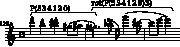
\includegraphics[scale=8]{sujeito-fugato}
    \label{fig:sujeito-fugato}
  }

  \subfigure[Counter-subject]{
    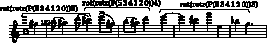
\includegraphics[scale=8]{contra-sujeito-fugato}
    \label{fig:contra-sujeito-fugato}
  }
  \caption{Structural elements of \eng{fugato}}
  \label{fig:elementos-fugato}
\end{figure}

\begin{figure}
  \centering
  \subfigure[Subject]{
    \includegraphics[scale=1]{output-subject}
    \label{fig:output-sujeito-fugato}
  }
  \subfigure[Counter-subject]{
    \includegraphics[scale=1]{output-countersubject}
    \label{fig:output-contra-sujeito-fugato}
  }
  \caption{Software output for \eng{fugato} contour operations}
  \label{fig:output-fugato}
\end{figure}


\end{multicols}
\end{center}


\begin{multicols}{3}

\section{The application of Contour in composition}

Systematic studies about the usage of contour operations and
combinations in musical composition are scarce, despite the possible
coherence that contours can provide. For this reason we are
researching the usage of contour in composition and its advantages.
The first author of this paper, during his master's
\cite{sampaio08:em}, composed a woodwind quintet,
% \textit{Em Torno da Romã}\footnote{Around the Pomegranate}
based on contour theories operations. We will use this piece as a case
study for the use of contour theory in composition, and how \goiaba{}
was useful in the compositional process.

% \textit{Em torno da Romã}
This piece
was composed entirely using \goiaba{} to simplify the calculation of
contour operations and plotting. The piece is based on the contour P(5
3 4 1 2 0) and on combinations of contour operations associated to
parameters such as pitch, tempo, density and texture. In figure
\ref{fig:c-534120} we can see the original contour P and its subsets
and operations; retrogradation, inversion, rotation, and
interpolation.

\goiaba{} was essential to compose a \eng{fugato} session in the
quintet because each part of the subject and countersubject were based
on different combinations of operations of rotation and
retrogradation. The subject is formed by the concatenation of P and
its rotation by a factor of 3, as seen in figure
\ref{fig:sujeito-fugato}. Figure~\ref{fig:output-sujeito-fugato} shows
\goiaba{}'s graphical output for both contours. The countersubject is
formed by a sequence of three rotations (by the factor of 5, 4, and 3)
of the retrograde of P (fig. \ref{fig:contra-sujeito-fugato}). We can
see the graphical output of these contours in figure
\ref{fig:output-contra-sujeito-fugato}.

\section{Conclusion and future work}

Contours help to give coherence to a musical piece, are easily
recognized graphically by musicians and laymen, and can be used to
analyze and compose music. Contour theories provide many operations
that demand precise mathematical calculations and graphical
representation, for this reason we are developing \goiaba{}, a contour
processing software that helps the calculation and plotting of contour
operations. \goiaba{} has been proven to be useful in composing music
that uses contour theory extensively. Currently \goiaba{} accepts only
input in a symbolic format, but we have plans to add support for
Lilypond, MIDI, ABC, and MusicXML formats as well. The next step in
our research is to improve \goiaba{} user interaction, releasing a
more friendly interface, possibly with a GUI.

\renewcommand{\refname}{References}

\bibliography{strings-short,computer-music,ismir,writing-style,harmonic-analysis,music-analysis,computational-musicology,melodic-contour,music-harmony-and-theory,programs,music-scores,genos}

\end{multicols}

\end{document}
